%% Copyright 2007-2020 Elsevier Ltd
%% 
%% This file is part of the 'Elsarticle Bundle'.
%% ---------------------------------------------
%% 
%% It may be distributed under the conditions of the LaTeX Project Public
%% License, either version 1.2 of this license or (at your option) any
%% later version.  The latest version of this license is in
%%    http://www.latex-project.org/lppl.txt
%% and version 1.2 or later is part of all distributions of LaTeX
%% version 1999/12/01 or later.
%% 
%% The list of all files belonging to the 'Elsarticle Bundle' is
%% given in the file `manifest.txt'.
%% 

%% Template article for Elsevier's document class `elsarticle'
%% with numbered style bibliographic references
%% SP 2008/03/01
%%
%% 
%%
%% $Id: elsarticle-template-num.tex 190 2020-11-23 11:12:32Z rishi $
%%
%%
\documentclass[final,a4paper]{elsarticle}
\usepackage[centering,top=1in,bottom=1in,left=1in,right=1in]{geometry}
\usepackage[dvipsnames]{xcolor}
\geometry{letterpaper}
% \documentclass[preprint,12pt]{elsarticle}

%% Use the option review to obtain double line spacing
%% \documentclass[authoryear,preprint,review,12pt]{elsarticle}

%% Use the options 1p,twocolumn; 3p; 3p,twocolumn; 5p; or 5p,twocolumn
%% for a journal layout:
%% \documentclass[final,1p,times]{elsarticle}
%% \documentclass[final,1p,times,twocolumn]{elsarticle}
%% \documentclass[final,3p,times]{elsarticle}
%% \documentclass[final,3p,times,twocolumn]{elsarticle}
%% \documentclass[final,5p,times]{elsarticle}
%% \documentclass[final,5p,times,twocolumn]{elsarticle}

%% For including figures, graphicx.sty has been loaded in
%% elsarticle.cls. If you prefer to use the old commands
%% please give \usepackage{epsfig}

%% The amssymb package provides various useful mathematical symbols
\usepackage{amssymb}
%% The amsthm package provides extended theorem environments
\usepackage{amsthm}
%% Include equations
\usepackage{amsmath}

\usepackage{bbm}

\usepackage{mathrsfs}
%% Include figures
\usepackage{graphicx}
\usepackage{float}
\usepackage{subfigure}
%% Enable clickable references
\usepackage[hidelinks]{hyperref}
%% For Table~s
\usepackage{setspace}
\usepackage{booktabs}
\usepackage{tabularx}
\usepackage[section]{placeins}

%% Include Figure~path
\graphicspath{{figures/}}

%% The lineno packages adds line numbers. Start line numbering with
%% \begin{linenumbers}, end it with \end{linenumbers}. Or switch it on
%% for the whole article with \linenumbers.
%% \usepackage{lineno}

\journal{Journal of the Mechanics and Physics of Solids}

% Flag to only show figures
\newif\ifincludetext
\includetexttrue
% Flag to only show figures

% Define new environment text

% \usepackage{comment}
% \ifincludetext
%   \newenvironment{text}[1][]
%   {}
% \else
%   \excludecomment{text}
% \fi

\begin{document}

\begin{frontmatter}

%% Title, authors and addresses

%% use the tnoteref command within \title for footnotes;
%% use the tnotetext command for theassociated footnote;
%% use the fnref command within \author or \address for footnotes;
%% use the fntext command for theassociated footnote;
%% use the corref command within \author for corresponding author footnotes;
%% use the cortext command for theassociated footnote;
%% use the ead command for the email address,
%% and the form \ead[url] for the home page:
%% \title{Title\tnoteref{label1}}
%% \tnotetext[label1]{}
%% \author{Name\corref{cor1}\fnref{label2}}
%% \ead{email address}
%% \ead[url]{home page}
%% \fntext[label2]{}
%% \cortext[cor1]{}
%% \affiliation{organization={},
%%             addressline={},
%%             city={},
%%             postcode={},
%%             state={},
%%             country={}}
%% \fntext[label3]{}

\title{Modeling intermittent laboratory earthquakes in rock gouge using rate-and-state friction with flash heating}

%% use optional labels to link authors explicitly to addresses:
%% \author[label1,label2]{}
%% \affiliation[label1]{organization={},
%%             addressline={},
%%             city={},
%%             postcode={},
%%             state={},
%%             country={}}
%%
%% \affiliation[label2]{organization={},
%%             addressline={},
%%             city={},
%%             postcode={},
%%             state={},
%%             country={}}

\affiliation[1]{organization={Mechanical and Civil Engineering, 
                    California Institute of Technology},%Department and Organization
            addressline={1200 E California Blvd}, 
            city={Pasadena},
            postcode={91125}, 
            state={CA},
            country={USA}}

\affiliation[2]{organization={Graduate Aerospace Laboratories, 
                                  California Institute of Technology},%Department and Organization
            addressline={1200 E California Blvd}, 
            city={Pasadena},
            postcode={91125}, 
            state={CA},
            country={USA}}
            
\affiliation[3]{organization={Seismological Laboratory, 
                                  California Institute of Technology},%Department and Organization
            addressline={1200 E California Blvd}, 
            city={Pasadena},
            postcode={91125}, 
            state={CA},
            country={USA}}
            

\author[1]{Shengduo Liu}
\author[1,3]{Nadia Lapusta}
\author[2]{Vito Rubino}
\author[2]{Ares Rosakis}

\begin{abstract}
%% Text of abstract
Destructive earthquake ruptures on natural faults occur as dynamic slip in layers of a fine granular material known as the fault gouge. 
An experimental study of earthquake ruptures within a Homalite-100 interface with fault gouge material has revealed the occurrence of complicated slip events, 
during which the dynamic slip initially arrests when it enters the fault gouge, 
then spontaneously and repeatedly re-nucleates and arrests within the gouge region \cite{Rubino2022}. 
The repeated strengthening and dramatic weakening of the fault gouge inferred by these experiments suggests that this behavior is due to velocity-strengthening properties at lower slip rates and dynamic-weakening, 
reminiscent of flash heating, at higher slip rates. 

To verify the conjectures based on the experimental results and to better understand the friction behavior within the fault gouge, 
we conduct 3-D finite-element simulations motivated by the lab experiments. 
In the experimental setup, 
dynamic ruptures are nucleated within the Homalite-100 interface and propagate there for a while before entering the fault gouge region.  
We assign velocity-weakening and velocity-strengthening rate-and-state properties to the Homalite-100 and gouge interface at low slip rates, 
respectively, 
coupled with strong dynamic-weakening effect at high slip rates.  
We find that the velocity-strengthening rate-and-state friction coupled with strong flash heating dynamic-weakening effect in the gouge region, 
is indeed able to first arrest the dynamic slip upon its arrival. 
However, 
we find that uniform friction with flash heating properties cannot achieve the experimentally-observed self-nucleation, 
and we have to introduce a patch that has a more efficient flash heating-like weakening and healing behavior at the location, 
which is physically motivated by shear localization and de-localization at the re-nucleation site due to accumulated slip. 

The simulation results indicate that the behavior of rupture propagation strongly depends on the initial slip rate over the fault, 
which calls for more holding experiments to narrow down the initial conditions. 
The simulations also reveal complex interactions between rupture on the Homalite-100 interface and the initially barrier-like gouge region, 
with the slip arrest in the gouge region propagating backward into the Homalite-100 interface, 
before the rupture elsewhere overtakes the rupture arrest and propagates forward into the gouge region again. 

\end{abstract}

%%Graphical abstract
% \begin{graphicalabstract}
% \includegraphics{grabs}
% \end{graphicalabstract}

%%Research highlights
\begin{highlights}
\item Research highlight 1
\item Research highlight 2
\end{highlights}

\begin{keyword}
%% keywords here, in the form: keyword \sep keyword
friction \sep 
dynamic-weakening \sep 
dynamic rupture simulations \sep 
rupture arrest \sep 
earthquake nucleation
% %% PACS codes here, in the form: \PACS code \sep code
% \PACS 0000 \sep 1111
% %% MSC codes here, in the form: \MSC code \sep code
% %% or \MSC[2008] code \sep code (2000 is the default)
% \MSC 0000 \sep 1111
\end{keyword}

\end{frontmatter}

%% \linenumbers

%% main text
%%%%%%%%%%%%%%%%%%%%%%%%%%%%%%%%%%%%%%%%%%%%%%%%%%%%%%%%%%%%%%%%%%%%%%%%%%%%%%%%%%%%%%%%%%%%%%
%                                        Introduction                                        %
%%%%%%%%%%%%%%%%%%%%%%%%%%%%%%%%%%%%%%%%%%%%%%%%%%%%%%%%%%%%%%%%%%%%%%%%%%%%%%%%%%%%%%%%%%%%%%
\section{Introduction}
\label{sec:introduction}
% Needs the following things:
%% More motivation and impact of FEM modeling
%% Literatures on the FEM simulations of frictional sliding
Understanding the underlying physics that control dynamic slip processes in natural rocks is crucial in earthquake-forecasting and reducing the potential damage. 
To study the complicated dynamic slip processes in geological faults that are usually non-homogeneous, 
Rubino et al. \cite{Rubino2022} conducted a lab experiment in which an initial slip event was triggered along the interface of two pre-stressed Homalite-100 plates by bursting an electric wire embedded in the interface. 
Part of the interface was set up to be the fault gouge zone with a different material to introduce non-homogeneous properties along it. 
After the initially triggered slip event was arrested upon entering the fault gouge zone, 
they observed intermittent dynamic slip events attempting to either enter from outside the fault gouge zone into it, 
or self nucleate within the fault gouge zone. 
Those experimental observations show that the fault gouge exhibits both an initial strengthening effect and afterwards a dynamic-weakening mechanism. 

Previous laboratory studies have shown that friction on Homalite-100 and fault gouge interfaces depend on the local slip rate and the slip history, 
as described by standard rate-and-state friction laws \cite{dieterich_modeling_1979, marone_laboratory-derived_1998}.
More specifically, 
rate-and-state velocity-strengthening interfaces have increasing steady-state friction coefficient as slip rate increases, 
which is consistent with the observed initial strengthening effect in the fault gouge in \cite{Rubino2022}, 
whereas velocity-weakening interfaces decrease their steady-state friction resistance as slip rate increases, 
which allow for runaway earthquakes and dynamic rupture propagation \cite{dieterich_modeling_1979, scholz_2019, rice_stability_1983}. 

As the slip rate along the fault gouge reaches the dynamic seismic level (around $1\ \mathrm{m/s}$), 
several dynamic-weakening mechanisms can be potentially activated, 
such as flash-heating, 
thermal-pressurization of pore fluids in the ambient gouge and bulk material, 
as well as shear-melting \cite{tsutsumi_high-velocity_1997, di_toro_friction_2004, beeler_constitutive_2008, tanikawa_frictional_2009, reches_fault_2010, faulkner_stuck_2011, goldsby_flash_2011, di_toro_fault_2011, kitajima_dynamic_2011, brown_melt_2012, proctor_dynamic_2014, boulton_high-velocity_2017, rowe_earthquake_2019, rice_heating_2006, noda_earthquake_2009}. 
These dynamic-weakening mechanisms, 
together with the initial strengthening effect due to rate-and-state velocity-strengthening friction properties, 
may explain the observed intermittent dynamic slip processes observed in \cite{Rubino2022}.

Motivated by the experiment in \cite{Rubino2022}, 
in this study, 
we conduct Finite Element (FE) simulations to model intermittent laboratory earthquakes in rock gouge using rate-and-state friction with flash heating dynamic-weakening mechanism. 
We explore the proper interface properties and / or loading conditions that can qualitatively reproduce the experimental observations, 
to foster better understanding of the complicated dynamic slip processes in non-homogeneous faults.

Section 2 introduces the problem setup, 
the physical and numerical model we use to simulate the intermittent earthquakes triggered in the lab experiment. 
Section 3 presents the numerical results of several representative cases using our modeling, 
with different interface properties as well as loading condition, 
and discusses possible explanations of the intermittent dynamic events observed in the lab experiment, 
including their arrest and re-nucleation. 
Finally, 
section 4 concludes the main findings of this study and gives insights on future directions of simulating intermittent lab earthquakes in fault gouges.


%%%%%%%%%%%%%%%%%%%%%%%%%%%%%%%%%%%%%%%%%%%%%%%%%%%%%%%%%%%%%%%%%%%%%%%%%%%%%%%%%%%%%%%%%%%%%%
%                              Problem Setup and Modeling                                    %
%%%%%%%%%%%%%%%%%%%%%%%%%%%%%%%%%%%%%%%%%%%%%%%%%%%%%%%%%%%%%%%%%%%%%%%%%%%%%%%%%%%%%%%%%%%%%%
\section{Problem Setup and Modeling}
\label{sec:problem}
% Geometry
In the experimental study on intermittent lab earthquakes with dynamic-weakening gouge \cite{Rubino2022},  
two pre-cut Homalite-100 blocks are compressed together at an angle as shown in Figure~\ref{fig:figureExp}(a) and Figure~\ref{fig:figure1}(a)(b), 
where part of the contact interface is made up of a type of fine-particle gouge material that has different frictional properties than the part of the interface with purely Homalite-100. 
To hold the fine particles in the gouge material, 
researchers set up a groove on each of the Homalite-100 blocks at the gouge region,
and put the gouge particles in the groove.
Therefore there is $1\ \mathrm{mm}$ Homalite wall surrounding the gouge region, 
as shown in Figure~\ref{fig:figure1}(b). 
In the experiment there were two explosive wires put on the interface to trigger dynamic slip events, 
as shown in Figure~\ref{fig:figureExp}(a), 
and they triggered two ruptures through bursting them individually. 
In this study, 
we focus on the first sequence of events after the first wire bursted, 
which is placed at $85\ \mathrm{mm}$ from the left edge of the interface. 

Figure~\ref{fig:figureExp}(b) shows the $x_1$-Time diagram of slip rate within the ``Field of View" as shown in (a). 
The color scale ranges from black at $0\ \mathrm{m/s}$, 
to red at $1\ \mathrm{m/s}$ and finally blue at $2\ \mathrm{m/s}$. 
Slip rates above $2\ \mathrm{m/s}$ will be shown as blue since they saturate the color scale. 
From (b) we can see the first rupture arriving at the interface at around $40\ \mathrm{\mu s}$ in two branches, 
one inter-sonic and one sub-Rayleigh. 
Then another self-contained event nucleates at around $85\ \mathrm{\mu s}$, $x_1 = 15\ \mathrm{mm}$, 
and is arrested shortly after. 
In our simulations, 
we try to understand the propagation of the two branches of the initial rupture, 
their arrest, 
and the re-nucleation and arrest of the second rupture in the gouge. 

The experiment also reveals first strengthening and then dynamic-weakening of friction in the gouge. 
Figure~\ref{fig:figureExp}(c) shows the evolution of friction with slip rate and slip from the experimental DIC measurements. 
It shows that as the rupture arrives at $x_1 = 8\ \mathrm{mm}$ in the gouge zone, 
the friction at the interface first increases, 
and then decreases dramatically as slip rate goes above $2\ \mathrm{m/s}$. 
This indicates that the friction of the gouge region first increases with slip rate, 
and then dynamically weakens as slip rate stays high. 


% ------------------------------- Experimental Figure~----------------------------------------
% Experimental results:
\begin{figure}[htbp]
    \centering
    \includegraphics[width=1.\textwidth]{figures/figure_exp_0327.pdf}
    \caption{Experimental setup and results from \cite{Rubino2022}. 
    (a) Homalite-100 plates with the $2\ \mathrm{mm}$ rock gouge layer in the experiment. The gouge particles are of micron meter length scale.
    (b) X-T diagram of slip rate measured in "Field of view" as shown in Figure~\ref{fig:figure1} through Digital-Image-Correlation. 
    After the first rupture arrives and gets arrested ($40$ to $50\ \mathrm{\mu s}$), 
    a profound event re-nucleates in the gouge layer at around $x_1 = 15\ \mathrm{mm}$, $t = 80\ \mathrm{\mu s}$. 
    (c) Friction coefficient and slip rate in the gouge layer at $x_1 = 8 \ \mathrm{mm}$ through DIC measurement at the front surface. 
    We clearly observe first strengthening effect,
    and then dynamic-weakening effect in the friction of the gouge,
    as ruptures propagate through.} 
    \label{fig:figureExp}
\end{figure}
% ------------------------------- Experimental Figure~----------------------------------------

% ---------------------------------------- Figure Modeling ------------------------------------------
\begin{figure}[htbp]
    \centering
    \includegraphics[width = 0.9\textwidth]{figure1.pdf}
    \caption{Geometry of the pre-cut Homalite-100 blocks and fault interface,  boundary and load conditions as well as the numerical approximation of wire-explosion triggering. 
(a) Finite element model inspired by the lab experiment in \cite{Rubino2022}. 2 pieces of pre-cut Homalite-100 samples ($\Omega$) are compacted together by unaxial load $P = 14.3$ $\mathrm{MPa}$ via a frictional interface ($I$). Part of the interface is modeled as rock gouge layer with different frictional properties than Homalite-100. The event of slip is triggered by introducing a normal stress perturbation along the interface motivated by wire explosion-triggering in the experiment. 
(b) Top view of the frictional interface with wire and rock gouge. The Homalite-100 and Rock gouge layer are modeled with velocity-weakening (VW) and velocity-strengthening (VS) rate-and-state friction models. Region 1 is Homalite-100 only while region 2 has gouge embedded in Homalite.
Note that viewing from the top, 
the gouge zone is surrounded by a thin-wall of Homalite at the front and back surfaces, 
due to the manufracture process of the sample. 
(c) Normal stress perturbation as a function of position ($x_1$) along the fault at time $t$. The symmetric trapezoid is centered at the wire position.
(d) Peak value of normal stress perturbation as a function of time $t$. Effective wire explosion time ($t=0$ $\mathrm{\mu s}$) is modeled as the first time $\sigma_{peak}$ reaches its maximum. 
Note that we do not have measured data for the explosion, and in this study, 
in general (unless specified otherwise), 
we adjust the explosion parameters to make sure the first rupture arrives at the ``Field of view" at around $40\ \mathrm{\mu s}$.}
    \label{fig:figure1}
\end{figure}
% --------------------------------------------------------------------------------------------

\FloatBarrier
% ~~~~~~~~~~~~~~~~~~~~~~~~~~~~~ Subsection physical modeling ~~~~~~~~~~~~~~~~~~~~~~~~~~~~~~~~~~~~~~~
\subsection{Physical modeling of the Homalite-100 plates and the interface with gouge}
Here we introduce the physical models we use in the Finite Element simulations for the Homalite-100 blocks and the fault interface. 

% Homalite-100 models
\subsubsection{Homalite-100 blocks: Linear elastic material}
It has been established that the pre-cut two pieces of Homalite-100 blocks in such experimental processes undergo small and approximately linear-elastic deformation \cite{rubino_understanding_2017}. 
However, 
the elastic constants used should be the set of parameters corresponding to the highly dynamic events \cite{rubino_understanding_2017}.

Then the governing equation of the Homalite-100 blocks is
\begin{align}
    G \boldsymbol{\nabla}^2 \boldsymbol{u}(\boldsymbol{x}, t) + \frac{G}{1 - 2\nu} \boldsymbol{\nabla} (\boldsymbol{\nabla} \cdot \boldsymbol{u}(\boldsymbol{x}, t)) = \rho \frac{d^2 \boldsymbol{u}(\boldsymbol{x}, t)}{d t^2}, \text{for}\ \boldsymbol{x} \in \Omega, \label{eq:Homalite},
\end{align}

\noindent where $\boldsymbol{u}(\boldsymbol{x}, t)$ is the displacement at location $\boldsymbol{x}$ and time $t$, 
$\rho$ is the mass density, 
$G$ is the shear modulus, 
and $\nu$ is the Poisson's ratio. 
The parameters we use in the simulations are listed in Table~\ref{tab:elasticPropsHomalite}.

% Friction model
\subsubsection{Fault constitutive model: Rate-and-state friction with flash heating effect}
Previous studies have found out that Homalite-100 interfaces have rate-and-state frictional properties with flash heating dynamic-weakening effect. 
In general, 
friction laws with rate-and-state dependence can be formulated by 

\begin{align}
    \tau(\boldsymbol{x}, t) &= f\left(V(\boldsymbol{x}, t), \theta(\boldsymbol{x}, t)\right) \sigma(\boldsymbol{x}, t), \text{for}\ \boldsymbol{x} \in I, \label{eq:generalFric} 
\end{align}

\noindent where $\tau(\boldsymbol{x}, t)$ is the shear stress, 
$\sigma(\boldsymbol{x}, t)$ is the corresponding normal stress, 
$V(\boldsymbol{x}, t)$ is the slip rate, 
and $\theta(\boldsymbol{x}, t)$ is the state variable at $\boldsymbol{x}$ and $t$.
The friction coefficient formulation $f(V, \theta)$ can include both rate-and-state dependence and flash heating effect. 
We adopt the formulation of rate-and-state friction by Dieterich \cite{dieterich_modeling_1979, ruina_slip_1983}. 
\begin{align}
    f_{RS}(V, \theta) &= f_* + a \log\left(\frac{V}{V_*}\right) + b \log\left(\frac{V_* \theta}{D_{RS}}\right) \label{eq:RS_friction}, 
\end{align}
where $f_*$, 
$V_*$ are reference friction coefficient and slip rate, 
$D_{RS}$ is the characteristic slip distance, 
$a$ and $b$ are non-dimensional rate-and-state parameters.

For the evolution law of the state variable $\theta$, 
unless otherwise stated, 
in this study we mainly adopt the ageing law \cite{dieterich_modeling_1979}. 
\begin{align}
    \frac{d\theta}{dt} &= 1 - \frac{V\theta}{D_{RS}} \label{eq:aging_law}. 
\end{align}
Another evolution law widely used for the state variable is the slip law \cite{ruina_slip_1983}, 
where 
\begin{align}
    \frac{d\theta}{dt} &=  - \frac{V\theta}{D_{RS}} \log\left(\frac{V\theta}{D_{RS}}\right) \label{eq:slip_law}. 
\end{align} 
We have comparisons between ageing and slip laws and would state explicitly when a case is run with slip law. 
When considering steady-state friction behavior, 
i.e. when $d\theta /dt = 0$, 
for both the ageing and slip law, 
we find

\begin{align}
    \theta^{ss} &= \frac{D_{RS}}{V_{ss}}, \label{eq:theta_ss}\\
    f_{RS}^{ss} &= f_* + (a-b) \log \left(\frac{V^{ss}}{V_*}\right). \label{eq:fRS_ss} 
\end{align}

\noindent This implies that when $a-b>0$, 
$f_{RS}^{ss}$ increases with $V^{ss}$, 
which is known as velocity-strengthening friction. 
Similarly,
if $a-b<0$,
the friction is velocity-weakening. 

Flash heating effect dynamically weakens the fault interface when it is slipping at high and seismic slip rates \cite{tsutsumi_high-velocity_1997, rice_heating_2006, beeler_constitutive_2008, goldsby_flash_2011}, 
in this study, 
we use the same flash heating formulation as \cite{Yuval_2020}:

\begin{align}
    f(V, \theta) &= f_w + \frac{f_{RS}(V, \theta) - f_w}{1 + D_{RS} / (\theta V_w)} \label{eq: flash_heating}, 
\end{align}

\noindent where $V_w$ and $f_w$ are flash heating slip rate and friction coefficient. 
Combining with (\ref{eq:theta_ss}), 
when the local slip rate is high, 
state variable $\theta$ is low and thus $f(V, \theta)$ goes to $f_w$, 
which is usually much smaller than half of the rate-and-state $f_*$. 
The friction parameters used for Homalite-100 interfaces are listed in Table~\ref{tab:fricPropsHomalite}, 
while the friction parameters for the Gouge zone is different by cases and will be discussed in the Results section.
% ~~~~~~~~~~~~~~~~~~~~~~~~~~~~~~~~~~ End of subsection ~~~~~~~~~~~~~~~~~~~~~~~~~~~~~~~~~~~~~~~

\FloatBarrier
% ~~~~~~~~~~~~~~~~~~~~~~ Subsection numerical modeling ~~~~~~~~~~~~~~~~~~~~~~~~~~~~~~~~~~~~~~~
\subsection{Numerical implementation of the physical modeling}
We build our finite element numerical model within the framework of PyLith, 
an open source Finite Element Library software with user-interface for new material and interface constitutive models \cite{Aagaard:Knepley:Williams:JGR:2013, PyLith:manual, PyLith:software}. 
For the elastic bodies, 
weak form of (\ref{eq:Homalite}) is solved explicitly under finite-element spatial discretization, 
with lumped mass matrix.  
The unknown traction at the fault interface are solved essentially as the Lagrangian multipliers to ensure both non-penetration condition in the fault-normal direction and friction constitutive relations in the fault-tangential directions. 
Denote the displacement at two sides of the interface of $I$ as $\boldsymbol{u}_{+}$ and $\boldsymbol{u}_{-}$. 
To advance the solution from $t_n$ to $t_{n+1} = t_n + \Delta t$, 
PyLith uses a prediction-correction scheme to enforce that the fault constitutive formulation is satisfied along the interface. 
First, 
it makes an initial attempt step with $\boldsymbol{u}^*(t_{n+1})$ solved with $\boldsymbol{u}_+^*(t_{n+1}) - \boldsymbol{u}_-^*(t_{n+1}) = 0$,  
i.e., 
no additional slip happens. 
That gives the required traction at the interface, 
both the shear component $\tau^*$ and the normal component $\sigma^*$, 
if no additional slip occurs. 
Then the governing equations of the fault interface, 
i.e. (\ref{eq:generalFric}, \ref{eq:aging_law}, \ref{eq: flash_heating}) are applied to modify the shear stress $\tau^*$, 
such that it satisfies the friction constitutive relations of the interface. 
Next, 
the displacement field is updated to reconcile the change in $\tau^*$ due to the modification step. 
The updated displacement field would change the required traction at $I$ to satisfy balance of linear momentum (\ref{eq:Homalite}), 
and also the friction coefficient if the friction coefficient depends on the slip history. 
PyLith loops the above process until both (\ref{eq:Homalite}) in $\Omega$ and (\ref{eq:generalFric}, \ref{eq:RS_friction}, \ref{eq: flash_heating}) are satisfied and report the corresponding displacement field as $\boldsymbol{u}(t_{n+1})$ \cite{PyLith:manual, PyLith:software}. 

We use rate-and-state aging law for the evolution of the state variable $\theta$, 
and to advance $\theta$ from $t$ to $t+\Delta t$, 
PyLith follows the scheme proposed by Kaneko et al. \cite{kaneko_spectral_2008, PyLith:manual}:

\begin{align}
    \theta(t_{n+1}) &= \theta(t_n)\exp\left(\frac{-V(t_n)\Delta t}{D_{RS}}\right) + \frac{D_{RS}}{V(t_n)}\left[1 - \exp\left(\frac{-V(t_n)\Delta t}{D_{RS}}\right)\right],  \label{eq:advancingTheta}
\end{align}

\noindent which essentially integrates (\ref{eq:aging_law}) from $t_n$ to $t_{n+1}=t_n + \Delta t$, 
assuming that $V$ is constantly $V(t_n)$. 
% ~~~~~~~~~~~~~~~~~~~~~~~~~~~~~~~~~~ End of subsection ~~~~~~~~~~~~~~~~~~~~~~~~~~~~~~~~~~~~~~~

%%%%%%%%%%%%%%%%%%%%%%%%%%%%%%%%%%%%%%%%%%%%%%%%%%%%%%%%%%%%%%%%%%%%%%%%%%%%%%%%%%%%%%%%%%%%%%
%                                 Results and discussion                                     %
%%%%%%%%%%%%%%%%%%%%%%%%%%%%%%%%%%%%%%%%%%%%%%%%%%%%%%%%%%%%%%%%%%%%%%%%%%%%%%%%%%%%%%%%%%%%%%
\section{Results and discussion}
\label{sec:resultsAndDiscussion}
In this section, 
we present and discuss the results of simulation cases with different friction properties, initial and loading conditions over the fault gouge region motivated by the experiment in \cite{Rubino2022}. 
Figure~\ref{fig:figureExp} shows the experimental setup and results from \cite{Rubino2022}.  
Slip at the front surface $x_3 = 0\ \mathrm{mm}$ is obtained through Digital-Image-Correlation (DIC). 
Then,
by differentiating in time and space, 
one can get the particle velocities and strains within the ``Field of View" as shown in Figure~\ref{fig:figure1}. 
Further,
assuming linear elasticity in the Homalite-100 plates, 
friction coefficient can be obtained. 
Figure~\ref{fig:figureExp}(a) shows the experimentally measured X-T diagram of slip rate at the front surface. 
At around $35\ \mathrm{\mu s}$ the first two ruptures marked by ``A" and ``B" arrives at the gouge region and gets arrested at $x_1 \approx 15\ \mathrm{mm}$. 
Then later at around $66\ \mathrm{\mu s}$ another rupture with a lower slip rate arrives and gets arrested again. 
Finally, 
at around $85\ \mathrm{\mu s}$, 
another dynamic rupture nucleates within the fault gouge region and is self-contained.
Figure~\ref{fig:figureExp}(b) shows the friction coefficient and slip rate vs. time at $x_1 = 8, 18\ \mathrm{mm}$, 
from which we observe that the friction coefficient initially strengthens as the rupture arrives, 
and then weakens as slip rate remains high. 

In the simulations, 
we explore and identify the parameters and conditions of the fault gouge that would lead to the experimental observations as shown in Figure~\ref{fig:figureExp}:
initial super-shear and sub-Rayleigh ruptures arriving at around $36, 40\ \mathrm{\mu s}$, 
and being arrested at $x_1 \approx 15\ \mathrm{mm}$. 
Then, 
a secondary dynamic rupture self nucleates at around $85\ \mathrm{\mu s}$ within the gouge region, 
and is self-contained. 
We start with a baseline model in \ref{subsec:baseline}, 
in which the entire interface has the friction and flash heating properties of Homalite-100, 
to verify that our finite element model is working properly, 
and we get the expected rupture propagation within the Homalite-100 interface. 
Then, 
in \ref{subsec:VSFHArrest} we specify velocity-strengthening with flash heating parameters for the fault gouge zone in Figure~\ref{fig:figure1}(b). 
The friction and flash heating parameters for the gouge zone are chosen based on point-wise measurements of slip rate and friction shown in Figure~\ref{fig:figureExp}(b). 
This time the initial rupture propagation is arrested, 
but there no secondary rupture nucleation can be observed because flash heating effect is largely not activated. 
To activate flash heating dynamic-weakening mechanism, 
in \ref{subsec:InitialCondition} we investigate the effect of initial condition in the fault gouge zone, 
and find that proper initial condition in the fault gouge zone can indeed activate flash heating and then self-nucleate a secondary rupture propagation within it. 

\FloatBarrier
% ~~~~~~~~~~~~~~~~~~~~~~~~~ Subsection: Baseline, no fault gouge ~~~~~~~~~~~~~~~~~~~~~~~~~~~~~
\subsection{Baseline: Purely velocity-weakening (VW) Homalite-100 interfaces cannot arrest dynamic ruptures} \label{subsec:baseline}
% ---------------------------- Case 1: Pure Homalite-100 Figure~------------------------------
% Case 1: Pure Homalite
\begin{figure}[htbp]
    \centering
    \includegraphics[width=1.\textwidth]{case1_wholefield_x3_0.pdf}
    \caption{Case 1, the fault interface has uniform Homalite-100 friction properties (no fault gouge is involved). 
    The initial slip rate over the entire interface is set to be $V_{initial}=10^{-7}\ \mathrm{m/s}.$
    The interface has uniform friction parameters and initial condition. 
    Shear, 
    pressure and Rayleigh wave speeds are marked as $c_s, c_p$ and $c_r$, 
    respectively.
    (a) $x_1$-Time diagram of slip rate. 
    (b) $x_1$-Time diagram of shear stress. 
    Note that the results are obtained at the front surface $x_3 = 0\ \mathrm{mm}$.
    We see that pure Homalite interface cannot arrest the initial rupture, 
    which starts as one sub-Rayleigh branch and then transits into a super-shear branch and a sub-Rayleigh branch, 
    consistent with observations in Figure~\ref{fig:figureExp}(b).}
    \label{fig:case1WholeFieldX3_0}
\end{figure}
% ---------------------------- Case 1: Pure Homalite-100 Figure~------------------------------
\ifincludetext {
As a baseline for further comparison, 
we first observe that the initiated rupture would propagate through the entire fault if it only has Homalite friction properties, 
i.e. rate-and-state velocity-weakening with flash heating effect \cite{rubino_understanding_2017}. 
Figure~\ref{fig:case1WholeFieldX3_0}, 
shows the result of this case, 
in which the entire fault interface has the Homalite-100 friction properties, 
as listed in Table~\ref{tab:fricPropsHomalite}. 
Since the entire fault interface is velocity-weakening (VW), 
the slip rate at the rupture tip increases as it propagates. 
Figure~\ref{fig:case1WholeFieldX3_0} shows the $x_1$-Time diagrams of slip rate and shear stress along the entire interface $x_1$, 
at the front surface where $x_3 = 0\ \mathrm{mm}$. 
Region 2 that contains the fault gouge inside is marked between the two red solid lines.
After the initial rupture starts at the wire, 
it first propagates in both directions at a sub-Rayleigh wave speed. 
Then after around $30\ \mathrm{\mu s}$,
the initial rupture transits into one sub-Rayleigh plus another super-shear wave propagation. 
The two rupture fronts with different wave speeds arrive at region 2 at approximately $36, 40\ \mathrm{\mu s}$, 
consistent with events "A" and "B" in the experiment as shown in Figure~\ref{fig:figureExp}. 
The ruptures get reflected at the two boundaries of the fault interface in $x_1$ direction. 
In the shear stress plot, 
we observe that at any $x_1$, 
the shear stress first rises when the rupture arrives, 
which is consistent with the rate-and-state direct effect \cite{dieterich_modeling_1979, Rice2001}. 
Then the shear stress drops significantly due to the flash heating (FH) dynamic-weakening mechanism imposed by (\ref{eq: flash_heating}).
Case 1 reflects how the wave propagates in the Homalite-100 region, 
which affects the evolution of shear stress and slip rate in the fault gouge. 
It also confirms that the transition of the initial rupture into two wave propagations, 
one sub-Rayleigh and one super-shear, 
happens before it reaches the fault gouge (region 2). 
This is consistent with the observed events ``A" and ``B" in the experiment. 
}
\fi

% ~~~~~~~~~~~~~~~~~~~~~~~~~~~~~~~~~~ End of subsection ~~~~~~~~~~~~~~~~~~~~~~~~~~~~~~~~~~~~~~~

\FloatBarrier
% ~~~~~~~~~~~~~~~~~~~~~~~~~ Subsection: VS+FH Fault gouge arrests ~~~~~~~~~~~~~~~~~~~~~~~~~~~~
%% SubSections: Fault gouge should be velocity-strengthening with flash heating mechanism
\subsection{Velocity-strengthening fault gouge can arrest the initial dynamic rupture} \label{subsec:VSNoFHArrest}
\ifincludetext{
To arrest the initial rupture propagating into the gouge zone, 
we further introduce velocity-strengthening friction (first without flash heating) properties for the fault gouge region in case 2. 
For the initial condition within the fault gouge region, 
creeping experiments 
% NEEDS REFERENCE
[ref. Pond] 
% NEEDS REFERENCE
suggest that depending on how long the Homalite-100 plates have been held together before the rupture is initiated in the experimental setting, 
the initial slip rate $V_{initial}$ ranges from $10^{-9}\ \mathrm{m/s}$ to $10^{-7}\ \mathrm{m/s}$.
Here we set $V_{initial}$ to be $10^{-7}\ \mathrm{m/s}$. 
The concrete parameters are listed in Table~\ref{tab:PropsGougeCases}. 
}
\fi

% ----------------------- Case 2: Homalite-100 + VS fault combined ----------------------------
\begin{figure}[htbp]
    \centering
    \includegraphics[width=1.\textwidth]{figures/case2_wholefield_x3_0_combined.pdf}
    \caption{Case 2, Homalite-100 with VS fault gouge simulation results. 
    The initial slip rate over the entire interface is set to be $V_{initial}=10^{-7}\ \mathrm{m/s}.$ 
    The plots have similar features as Figure~\ref{fig:case1WholeFieldX3_0}. 
    (a) $x_1$-Time diagram of slip rate, measured at $x_3 =0\ \mathrm{mm}$.
    (b) $x_1$-Time diagram of shear stress, measured at $x_3 =0\ \mathrm{mm}$.
    (c) $x_1$-Time diagram of slip rate \textbf{differences} between $x_3 = -5\ \mathrm{mm}$ and $x_3 = 0\ \mathrm{mm}$, 
    note that the color scale is changed to $[-2, 2]\ \mathrm{m/s}$ to show that the difference is small.
    (d) $x_1$-Time diagram of shear stress, measured at $x_3 =0\ \mathrm{mm}$.
    The gouge layer with velocity-strengthening friction properties can arrest the initial rupture upon its arrival. 
    A secondary rupture arrives at the gouge layer at around $80\ \mathrm{\mu s}$. 
    We also notice that the slip-rate difference in $x_3$ direction is not significant compared to its magnitude, 
    while the difference in shear stress is significant due to the transition from velocity-weakening Homalite to velocity-strengthening gouge, 
    as $x_3$ decrease from $0\ \mathrm{mm}$ to $-5\ \mathrm{mm}$.}
    \label{fig:case2WholeFieldX3_combined}
\end{figure}
% ----------------------- Case 2: Homalite-100 + VS fault combined ----------------------------
\ifincludetext {
Figure~\ref{fig:case2WholeFieldX3_combined} (a)(b) are the $x_1$-Time diagram of slip rate and shear stress at the $x_3 = 0\ \mathrm{mm}$ for case 2, 
from which we can see that the right branch of rupture gets arrested due to the velocity-strengthening property of the fault gouge. 
Then later at around $90\ \mathrm{\mu s}$, 
another rupture enters region 2 from the Homalite-100 region and is impaired again by the fault gouge. 
The shear stress plot shows that the region where the rupture reaches experiences flash heating weakening. 
Since the shear stress is plotted at the front surface $x_3 = 0\ \mathrm{mm}$, 
where the material at the interface is still Homalite-100, 
we do not see the velocity-strengthening effect. 
Figure~\ref{fig:case2WholeFieldX3_combined} (c)(d) shows the $x_1$-Time diagrams of slip rate difference and shear stress for case 2,
in the middle of the fault $x_3 = -5\ \mathrm{mm}$. 
Slip rate difference with respect to $x_3 = 0\ \mathrm{mm}$ is plotted in (c) to verify that slip rate does not vary much in $x_3$ direction. 
Note that the color scale is $[-2, 2]\ \mathrm{m/s}$ in (c), 
while it is $[0, 15]\ \mathrm{m/s}$ in (a). 
In contrast to the small difference in slip rate between $x_3 = 0\ \mathrm{mm}$ and $-5\ \mathrm{mm}$, 
we notice that the shear stress in (d) indeed shows velocity-strengthening effect, 
since we are looking at the gouge zone of the interface.


We have validated that the velocity-strengthening fault gouge can arrest the initial dynamic rupture propagation. 
However, 
since no dynamic-weakening effect such as flash heating is included in the gouge zone, 
physically it is unlikely to re-nucleate a secondary rupture within it. 
Next we incorporate flash-heating like dynamic-weakening mechanism that foster self-nucleation of dynamic ruptures in the fault gouge, 
as observed in the experiments. 
Note that the second rupture arriving at the gouge zone at around $80\ \mathrm{\mu s}$ is not a self-nucleation but a rupture coming from the Homalite portion of the interface. 
}
\fi

\FloatBarrier
%% SubSections: Fault gouge should be velocity-strengthening with flash heating mechanism
\subsection{Velocity-strengthening with flash-heating dynamic-weakening fault promotes a secondary rupture in the gouge} \label{subsec:VSFHArrest}
\ifincludetext{
As we further include flash heating dynamic-weakening effect in the gouge zone, 
we see more dynamic rupture propagation, 
which can potentially lead to self-nucleation. 
Figure~\ref{fig:case3WholeFieldX3_combined} plots slip rate and shear stress for the case with velocity-strengthening plus flash heating gouge, 
in similar fashion as Figure~\ref{fig:case2WholeFieldX3_combined}. 
All other parameters are kept the same as case 2. 
Slip rate is larger compared to case 2 because of flash heating effect, 
which is evident from the shear stress decrease in the gouge zone,  
shown in (d). 
Note that in (a), 
we see some intermittent increase and decrease in the slip rate, 
and this is due to the waves transversing in $x_3$ direction, 
which will be illustrated later with a comparison with a 2D simulation. 
Note that the secondary rupture still comes back to the gouge zone at around $80\ \mathrm{\mu s}$ from the Homalite region of the interface. 
}

% ----------------------- Case 3: Homalite-100 VS + FH fault combined ----------------------------
\begin{figure}[htbp]
    \centering
    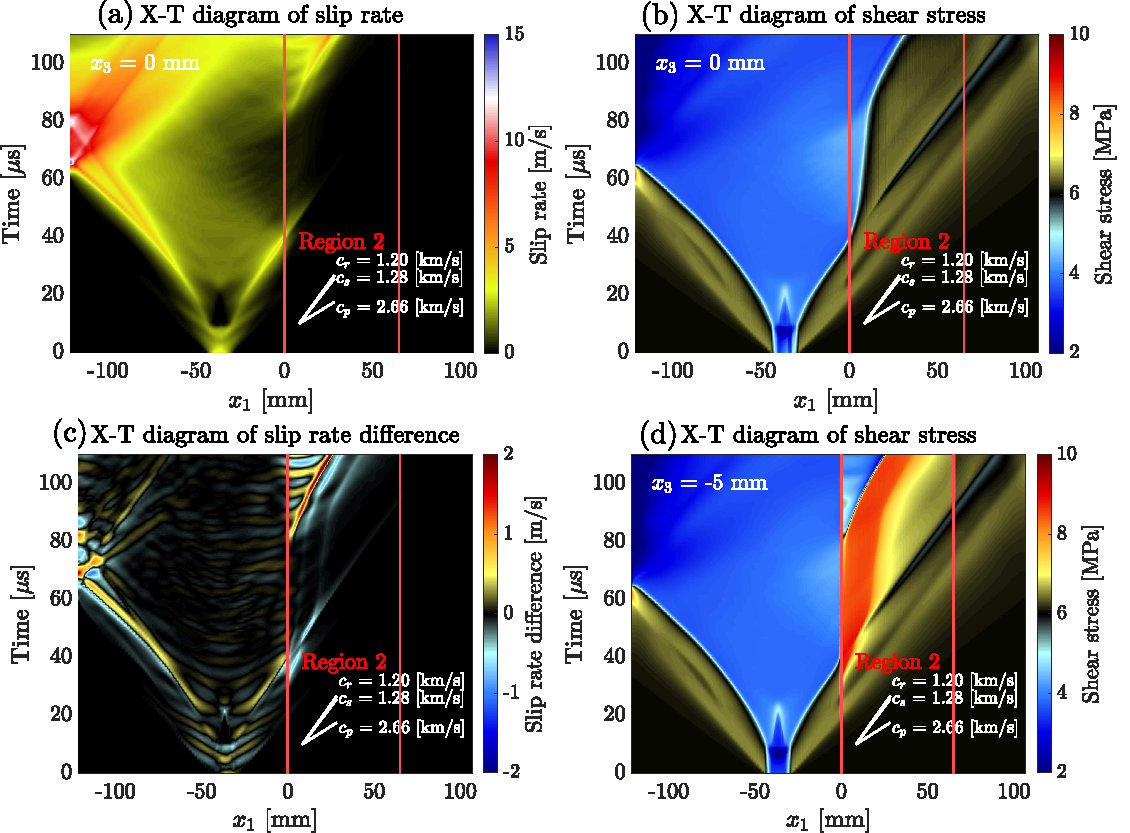
\includegraphics[width=1.\textwidth]{figures/case3_wholefield_x3_0_combined_VSFH.pdf}
    \caption{Case 3, Homalite-100 with VS and FH fault gouge simulation results. 
    The initial slip rate over the entire interface is set to be $V_{initial}=10^{-7}\ \mathrm{m/s}.$ 
    The plots have similar features as Figure~\ref{fig:case2WholeFieldX3_combined}. 
    (a) $x_1$-Time diagram of slip rate, measured at $x_3 =0\ \mathrm{mm}$.
    (b) $x_1$-Time diagram of shear stress, measured at $x_3 =0\ \mathrm{mm}$.
    (c) $x_1$-Time diagram of slip rate \textbf{differences} between $x_3 = -5\ \mathrm{mm}$ and $x_3 = 0\ \mathrm{mm}$, 
    note that the color scale is changed to $[-2, 2]\ \mathrm{m/s}$ to show that the difference is small.
    (d) $x_1$-Time diagram of shear stress, measured at $x_3 =0\ \mathrm{mm}$. 
    We observe that further adding flash-heating (FH) dynamic-weakening effect allows for a more dynamic secondary rupture at around $80\ \mathrm{\mu s}$. 
    In (d) we see that the shear resistance of the gouge layer first strengthens and then dynamically weakens due to the imposed FH effect.}
    \label{fig:case3WholeFieldX3_combined}
\end{figure}
% ----------------------- Case 3: Homalite-100 + VS FH fault combined----------------------------

\ifincludetext{
As a comparison between the experiment and the simulation cases with pure Homalite (no gouge), 
velocity-strengthening gouge and velocity-strengthening gouge further equipped with flash heating effect, 
Figure~\ref{fig:EXPHMVSFH} shows the slip rate within the experimental ``Field of View" at $x_3 = 0\ \mathrm{mm}$. 
We observe that with uniform Homalite and gouge friction properties, 
we are able to reproduce the arrival and arrest of the first rupture propagation around $40\ \mathrm{\mu s}$. 
Further with velocity-strengthening plus flash heating gouge friction properties, 
we are able to obtain a secondary rupture that has the same slip rate as the experiment. 
However, 
the second rupture arrives from the Homalite zone and is not self-contained, 
as in the experiment. 
}
\fi

% ----------------------- Case experiment, 1, 2, 3 Slip rate ----------------------------
\begin{figure}[htbp]
    \centering
    \includegraphics[width=1.\textwidth]{figures/EXP_HMOnly_VSNOFH_VSFH.pdf}
    \caption{$x_1$-Time diagrams of slip rates within the ``Field of View" from the experiment, Homalite-only interface (case 1), Homalite with velocity-strengthening (VS) gouge (case 2), Homalite with VS and flash-heating (FH) gouge (case 3). 
    Note that here the color scale is $[0, 2]\ \mathrm{m/s}$. 
    Velocity-strengthening with flash heating gouge can arrest the initial rupture. 
    It also allows for a secondary rupture with rupture speed consistent with the experimental results. 
    However, 
    with uniform friction properties in the gouge layer, 
    the secondary rupture does not self-nucleate or get arrested afterwards.}
    \label{fig:EXPHMVSFH}
\end{figure}
% ----------------------- Case experiment, 1, 2, 3 Slip rate ----------------------------
\ifincludetext{
The shear stress varies significantly with $x_3$ because of the transitioning from Homalite to gouge and finally Homalite again as $x_3$ decreases from $0$ to $-5\ \mathrm{mm}$. 
Figure~\ref{fig:EXPStressX3} shows the $x_1$-Time diagrams of shear stress comparison between the experiment and $x_3 = \{0, -2, -5\}\ \mathrm{mm}$ in case 3. 
From it we observe that the experimental shear stress measurement, 
though obtained from displacement field within ``Field of View" at $x_3 = 0\ \mathrm{mm}$, 
has both increased and decreased shear stress as the rupture propagates. 
Since at $x_3 = 0\ \mathrm{mm}$ the interface material is Homalite only, 
which is velocity-weakening, 
there should not be any increased shear stress observed. 
Thus it is possible that the experimental results of shear stress is a combination of shear stress through all $x_3\in [-10, 0]\ \mathrm{mm}$.  
This is potentially because the DIC method requires the displacement field to be continuous, 
and so the slip at the fault interface is computed through some extrapolation from a distance above or below it. 
This distance is related to the window size used in the specific DIC algorithm. 
}
\fi
% ----------------------- Case 3 shear stress at different x3 ----------------------------
\begin{figure}[htbp]
    \centering
    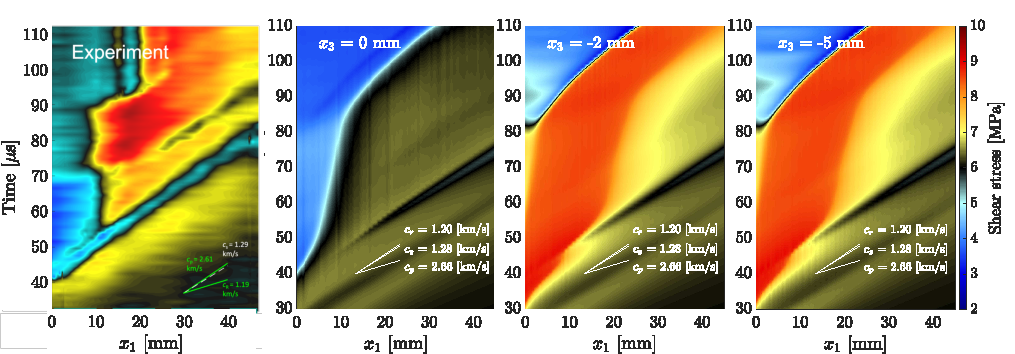
\includegraphics[width=1.\textwidth]{figures/EXP_Stress_x3.pdf}
    \caption{$x_1$-Time diagrams of shear stress within the ``Field of View" from the experiment and case 3 at different $x_3$. 
    The experimental measurement is likely a combination of the shear stress at different $x_3$'s, 
    as a result of the DIC-algorithm extrapolated to the fault interface.}
    \label{fig:EXPStressX3}
\end{figure}
% ----------------------- Case 3 shear stress at different x3 ----------------------------

\ifincludetext{
To check that the small-scale oscillations in case 3 with velocity-strengthening plus flash heating gouge, 
as shown in the right-most panel in Figure~\ref{fig:EXPHMVSFH}, 
is physical rather than numerical, 
we run it with three different mesh sizes and check mesh convergence. 
Figure~\ref{fig:meshConv} shows the friction coefficient, 
slip rate and slip vs. time, 
for three different meshes of edge length $2, 0.5, 0.1\ \mathrm{mm}$, 
respectively. 
We first confirm that the oscillations in the results are indeed physical, 
due to the good mesh convergence shown. 
We also see the friction coefficient first increases due to the velocity-strengthening property of the gouge, 
and then decreases due to flash heating dynamic-weakening mechanism. 
}
\fi
% --------------------------------- Case 3 mesh convergence ----------------------------------
% Case 3 mesh convergence
\begin{figure}[htbp]
    \centering
    \includegraphics[width=1.\textwidth]{figures/figure_meshconv_0327.pdf}
    \caption{Case 3, friction coefficient, slip rate and slip vs. time at $x_3 = -5 \mathrm{mm}$. 
    Mesh 1, 2, 3 have mesh edge-lengths of around $2, 0.5, 0.1\ \mathrm{mm}$, respectively.
    The friction coefficient first increases due to the velocity-strengthening property of the gouge, 
    and then decreases due to flash-heating effects.}
    \label{fig:meshConv}
\end{figure}
% --------------------------------- Case 3 mesh convergence ----------------------------------

\ifincludetext{
To check whether using slip law for the evolution of state variable $\theta$ would give us qualitatively different results, 
we run a case with velocity-strengthening gouge plus flash heating effect, 
in which the evolution for the state variable along the fault obeys the slip law as stated in (\ref{eq:slip_law}). 
Figure~\ref{fig:SLPatchCombined} shows the $x_1$-Time diagrams of slip rate, 
as well as the evolution of slip rate vs. time and friction coefficient vs. slip, 
for ageing and slip law. 
We see that the rupture behavior is not qualitatively different, 
with both laws arresting the first rupture and the second rupture arriving from the Homalite. 
Note that under the same explosion condition, 
the case with slip law requires larger $D_{RS}$, 
as also mentioned by \cite{Yuval_2020}. 
From the Friction coefficient vs. slip plot, 
one can also verify that the two laws have similar cohesive energy (proportional to the area-under-curve), 
and thus behaves similarly under the same explosion. 
}
\fi
% --------------------------------- Case 3 Ageing vs. Slip ----------------------------------
% Case 3 mesh convergence
\begin{figure}[htbp]
    \centering
    \includegraphics[width=1.\textwidth]{figures/AgeingVsSlip_VF.pdf}
    \caption{Comparison between ageing and slip law for case 3. 
    The upper two $x_1$-Time plots of slip rates are under the same parameters as case 3 (shown in Figure~\ref{fig:case3WholeFieldX3_combined}(a)). 
    The below plots show Slip rate vs. Time (left 2) and Friction coefficient vs. Slip (right 2), 
    in the Homalite ($x_1 = -50\ \mathrm{mm}$) and in the gouge ($x_1 = 5\ \mathrm{mm}$). 
    The difference is not significant qualitatively.}
    \label{fig:AgeingVsSlipCase3}
\end{figure}
% --------------------------------- Case 3 Ageing vs. Slip ----------------------------------

% ~~~~~~~~~~~~~~~~~~~~~~~~~~~~~~~~~~ End of subsection ~~~~~~~~~~~~~~~~~~~~~~~~~~~~~~~~~~~~~~~

\FloatBarrier
% ~~~~~~~~~~~~~~~~~~~~~~~ The behavior of the secondary rupture depends significantly on the initial condition over the interface ~~~~~~~~~~~~~~~~
\subsection{The behavior of the secondary rupture depends significantly on the initial slip rate over the interface} \label{subsec:InitialCondition}
\ifincludetext{
To testify the sensitivity of our simulations results on the initial condition over the interface, 
i.e. the initial slip rate, 
based on relevant evidence from interface-holding-experiments (cite pond here), 
we keep the same interface property with velocity-strengthening plus flash heating effect, 
and in addition to running case 3 with $V_{initial} = 10^{-7}\ \mathrm{m/s}$, 
we run two more cases with $V_{initial} = 10^{-8}\ \mathrm{m/s}$ and $V_{initial} = 10^{-9}\ \mathrm{m/s}$. 
By the rate-and-state formulation shown in (\ref{eq:RS_friction}), 
we can compute the required initial value for the state variable $\theta$ by

\begin{align}
    \theta_{initial} &= \frac{D_{RS}}{V_*}
    \exp{\left(\frac{\tan(\alpha) - f_* - a\log(V_{initial}/V_*)}{b}\right)}. \label{eq:estimate_theta_initial}
\end{align}

If we keep the explosion condition unchanged. 
Figure~\ref{fig:VInitialConstExplosion} shows the slip rate for those three different $V_ini$s. 
It is clear that under the same explosion, 
reducing the initial slip rate would significantly delay the arrival of the initial rupture. 
Since we cannot directly measure the explosion, 
this suggests it necessary to conduct further experiments on setting the initial condition over the interface. 
}
\fi
% -------------------------------------- Dependence on V_ini, not adjusting explosion  ---------------------------------------
\begin{figure}[htbp]
    \centering
    \includegraphics[width=1.0\textwidth]{figures/V_initial_explosion_const.pdf}
    \caption{$x_1$-Time diagrams of slip rates in the observation window for $V_{initial} = 10^{-7}\ \mathrm{m/s}$, 
    $V_{initial} = 10^{-8}\ \mathrm{m/s}$, 
    $V_{initial} = 10^{-9}\ \mathrm{m/s}$. 
    Here the three cases have the same explosion conditions and friction parameters. 
    We can see that under the same explosion, 
    Reducing the initial slip rate would delay the arrival time of the initial rupture, 
    and finally not even nucleate the initial rupture propagation. 
    This suggests further experiments on setting the initial slip rate be necessary to study the intermittent lab earthquakes in detail.
    }
    \label{fig:VInitialConstExplosion}
\end{figure}
% -------------------------------------- Dependence on V_ini, not adjusting explosion  ---------------------------------------

% -------------------------------------- Dependence on V_ini, adjusting explosion  ---------------------------------------
\begin{figure}[htbp]
    \centering
    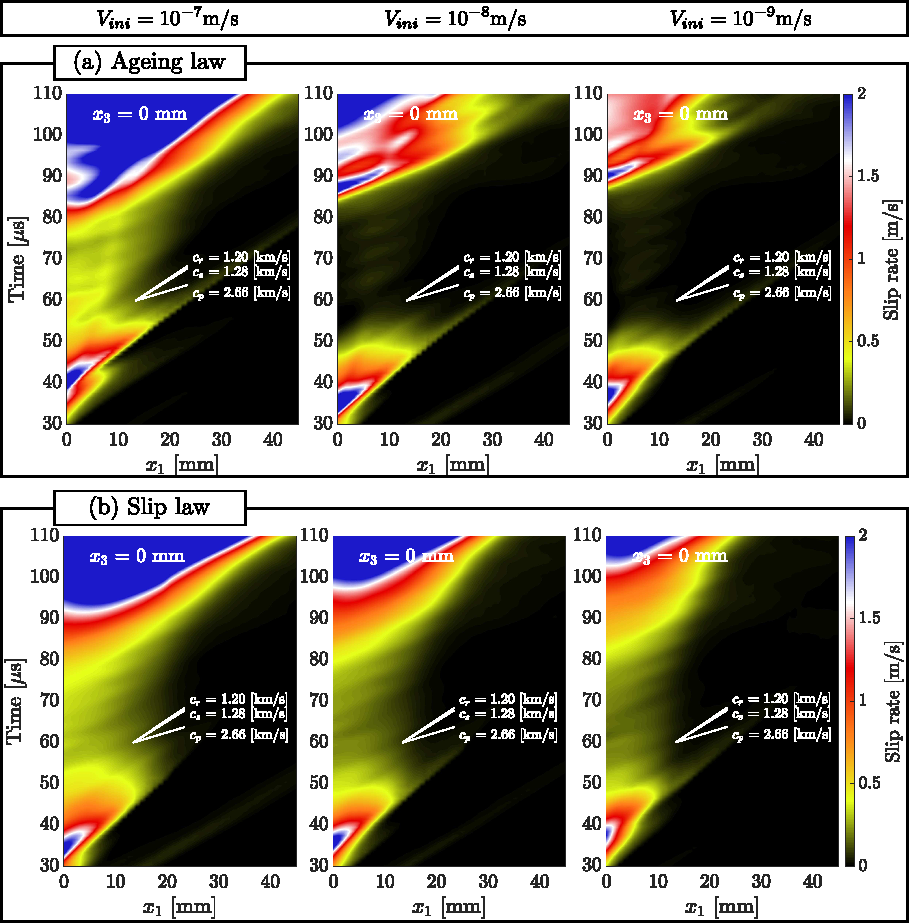
\includegraphics[width=1.0\textwidth]{figures/V_initial_ageing_slip.pdf}
    \caption{$x_1$-Time diagrams of slip rates in the observation window for $V_{initial} = 10^{-7}\ \mathrm{m/s}$, 
    $V_{initial} = 10^{-8}\ \mathrm{m/s}$, 
    $V_{initial} = 10^{-9}\ \mathrm{m/s}$, 
    for both ageing (a) law and (b) slip law. 
    Here we tune the explosion parameters such that the first rupture arrives in the gouge zone at around $30$ to $40\ \mathrm{\mu s}$, 
    to be consistent with the experiment in Figure~\ref{fig:figureExp}(b).
    Reducing the initial slip rate over the interface would make the secondary rupture significantly less dynamic. 
    However, 
    the secondary rupture enters the ``Field of view" at around $80$~$90\ \mathrm{\mu s}$ in all six cases. 
    Slip law has more smooth ruptures because the required $D_{RS}$ is larger.}
    \label{fig:VInitialAdjustedExplosion}
\end{figure}
% -------------------------------------- Dependence on V_ini, adjusting explosion  ---------------------------------------
\ifincludetext{
Conditioned on the fact that the first rupture arrives at the gouge layer at around $40\ \mathrm{\mu s}$, 
we study whether by adjusting the explosion to ensure that, 
different initial slip rates would give us qualitatively similar results. 
Figure~\ref{fig:VInitialAdjustedExplosion} shows the $x_1$-Time diagrams of slip rate for different slip rates, 
with the explosion adjusted to ensure first rupture arrival time, 
for both ageing and slip law. 
It is clear that for both laws, 
the second rupture becomes much less dynamic as the initial slip rate reduces from $10^{-7}$ to $10^{-9}\ \mathrm{m/s}$. 
Ageing and slip law produce qualitatively similar results, 
with the slip law having more smooth profiles because of larger $D_{RS}$ to achieve similar cohesive energy. 
We also notice that even if the second rupture is significantly impaired by reduced slip rate, 
in all the cases it starts re-entering the gouge zone at around $80\ \mathrm{\mu s}$, 
which has not been observed in the experiment. 
}
\fi

% ~~~~~~~~~~~~~~~~~~~~~~~~~~~~~~~~~~ End of subsection ~~~~~~~~~~~~~~~~~~~~~~~~~~~~~~~~~~~~~~~
\FloatBarrier
% ~~~~~~~~~~~ Self-nucleation through a more-efficient weakening patch  ~~~~~~~~~~~~~~~~~~~~~~~~~~~~~~~~~~~~~~~
\subsection{Self-nucleation by introducing a more-efficient weakening patch in the gouge zone} \label{subsec:selfNucleation}
\ifincludetext{
From the cases shown above, 
we observe that gouge with velocity-strengthening plus flash heating friction properties is able to arrest the first rupture arriving at the interface at around $40\ \mathrm{\mu s}$, 
and then a second rupture enters from the Homalite region into the gouge at around $80\ \mathrm{\mu s}$, 
and is never arrested.  
However, 
in the experimental result shown in Figure~\ref{fig:figureExp}, 
the second rupture self-nucleates within the gouge zone, 
and is arrested shortly after nucleated. 
We have tried cases with different explosion parameters, 
friction parameters, initial conditions, etc., 
and find that with uniform friction properties in the Homalite and gouge zone respectively, 
under our formulation of (\ref{eq:RS_friction}, \ref{eq: flash_heating}), 
the second rupture would come back from the Homalite instead of self-nucleating in the gouge. 
Also the flash heating by (\ref{eq: flash_heating}) makes the second rupture difficult to be arrested once initiated. 
With those considered, 
here we propose non-uniform friction properties along the interface to fully recover the experimental results.
}
\fi

\ifincludetext{
To nucleate a self-contained second rupture at about $x_1 = 15\ \mathrm{mm}$, 
we introduce a $V_w$-weakening-healing patch in the gouge zone. 
Figure~\ref{fig:SLPatchCombined}(a) shows the position of the patch. 
The slip-weakening and slip-healing feature of $V_w$ is shown by (b). 
Based on the flash-heating formulation (\ref{eq: flash_heating}), 
this would make friction coefficient $f(V, \theta)$ easier to decrease to the flash heating weakened value $f_w$. 
To arrest the second rupture shortly after its nucleation, 
$V_w$ would heal if more slip happens at the patch. 
Since the uniform velocity-weakening Homalite interface would result in a strong coming-back rupture at around $80\ \mathrm{\mu s}$, 
we further introduce a region (as shown in Figure~\ref{fig:SLPatchCombined}(a)) to the left of the wire that has different rate-and-state properties to impair the left rupture branch shown in Figure~\ref{fig:case3WholeFieldX3_combined}(a). 

With the partly-strengthened Homalite and the $V_w$ patch, 
we run two cases (ageing and slip law, respectively) with $V_{initial} = 10^{-7}\ \mathrm{m/s}$. 
Figure~\ref{fig:SLPatchCombined}(c) shows the self-nucleation and arrest of the second event. 
Note that both of them are qualitative similar to the experimental result in Figure~\ref{fig:figureExp}(a), 
while the case with slip law is run with $V_w^{low}=0.1\ \mathrm{m/s}$, 
which is more consistent with previous studies [cite Rice]. 
Figure~\ref{fig:SLPatchCombined}(d) and (e) shows the nucleation and arrest process within the patch for slip law. 
We clearly see that a dynamic event nucleates in the gouge zone and then spreads to the front surface. 
As the patch heals, 
shear stress recovers and slip rate drops down. 
This result suggests that a localization-delocalization process in the gouge region possibly causes the self nucleation and arrest observed in the experiment. 

An important remark here is that the surrounding Homalite region of the gouge zone is crucial to the self-nucleation, 
because for $V_w$ to decrease to its low value, 
the cumulative slip at the location needs to reach several microns, 
and the surrounding Homalite region fosters slip in the patch. 
We have run a case without the surrounding Homalite region and under the same explosion, initial condition and friction parameters, 
no self-nucleation can be achieved. 

}
\fi
% --------------------------------- Self nucleation ----------------------------------
% Patch to achieve self nucleation
\begin{figure}[htbp]
    \centering
    \includegraphics[width=1.0\textwidth]{figures/SL Patch_AgeingSlipCombined.pdf}
    \caption{Self nucleation can be achieved by blocking the left branch of the initial rupture within the Homalite, and introducing a more efficient $V_w$-slip weakening patch within the gouge layer. 
    (a) The Homalite section to the left of the wire is set to be velocity-strengthening, to block the left branch of the initial rupture. A $V_w$ slip weakening patch is pput in the gouge zone. 
    (b) The weakening of $V_w$ vs. slip in the patch follows the piecewise linear fashion.
    (c) The X-T diagrams of slip rate for cases without and with the slip-weakening patch. 
    The case without the patch shows that the VS Homalite section is able to prevent the secondary rupture from entering the gouge zone at around $90\ \mathrm{\mu s}$, 
    while the case with the patch achieves self-nucleation by its more efficient weakening. 
    (d) Snapshots of slip rate at the interface at $78.45, 82.45, 86.45, 90.45\ \mathrm{\mu s}$, 
    for the case with Slip law. 
    From it we can clearly see the self-nucleation process and its arrest later. 
    (e) Snapshots of shear stress at the interface at $78.45, 82.45, 86.45, 90.45\ \mathrm{\mu s}$, 
    for the case with \textbf{slip law}. 
    Shear stress first decreases in the patch and then recovers, due to the evolution of $V_w$ with slip as in (b).}
    \label{fig:SLPatchCombined}
\end{figure}
% --------------------------------- Self nucleation ------------------------------------------
% ~~~~~~~~~~~~~~~~~~~~~~~~~~~~~~~~~~ End of subsection ~~~~~~~~~~~~~~~~~~~~~~~~~~~~~~~~~~~~~~~

\FloatBarrier
% ~~~~~~~~~~~~~~~~~~~ Comparing 3D and 2D simulations  ~~~~~~~~~~~~~~~~~~~~~~~~~~~~~~~~~~~~~~~
\subsection{Comparing 3D and 2D simulations} \label{subsec:3Dvs2DSimulations}
\ifincludetext{
Since the specimen is $200\ \mathrm{mm}$ long and wide, 
but only $10\ \mathrm{mm}$ thick, 
a natural question to ask is how much feature we will be able to capture just with a 2D simulation in plane-stress. 
We here run a case with the same material parameters and initial condition as case 3 in 2D. 
However, 
in 2D simulation there will be no Homalite region surrounding the gouge zone as the 3D simulation, 
since $x_3$ direction does not exist. 
It turns out that the surrounding Homalite region makes it easier for the rupture to propagate, 
and the difference is noticable. 
}
\fi
% ------------------------------------ With 2D simulations -----------------------------------
% Full field comparison of 2D and 3D at Vini=10^-7
\begin{figure}[htbp]
    \centering
    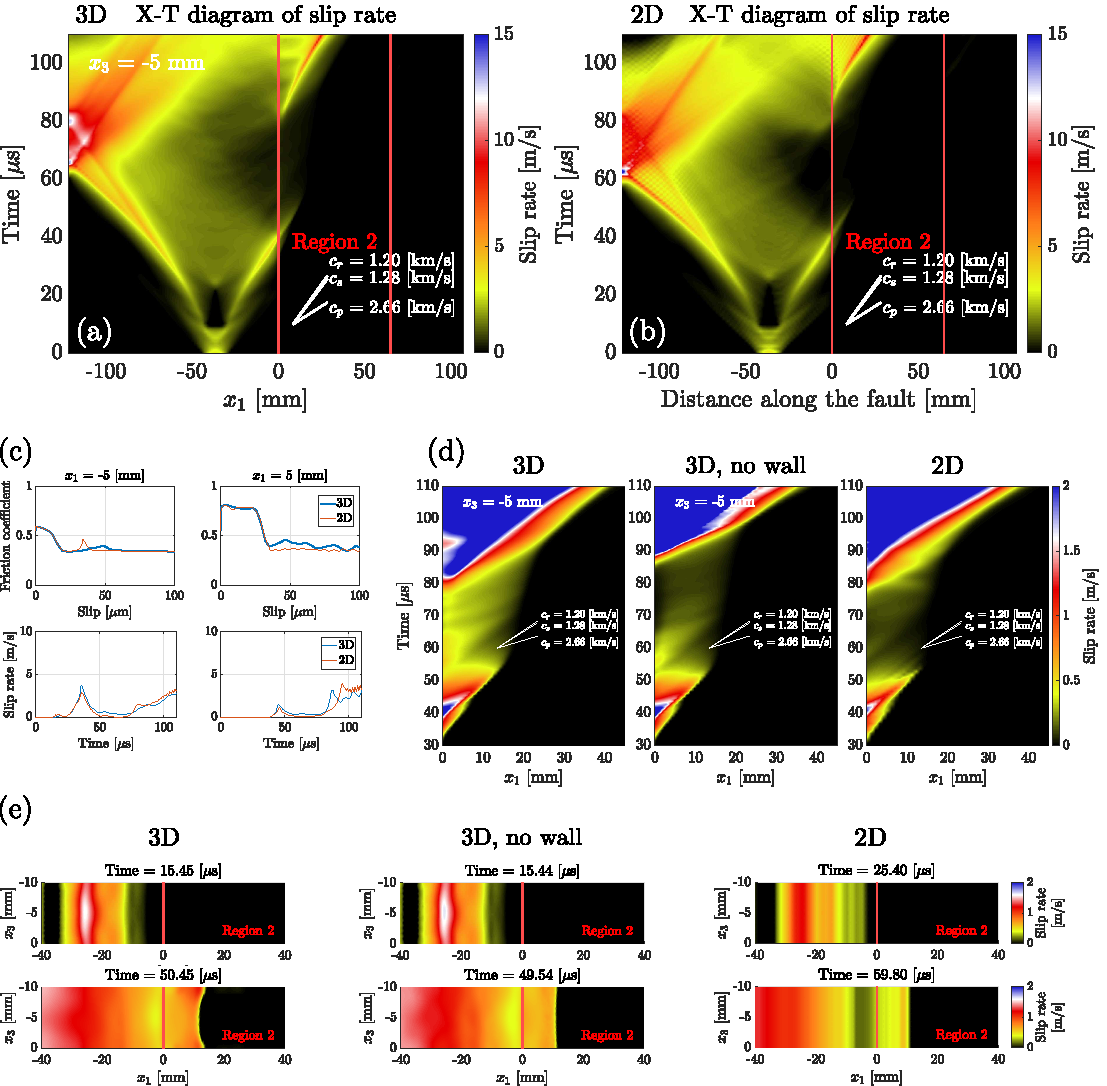
\includegraphics[width=1.0\textwidth]{figures/2Dvs3D_full.pdf}
    \caption{(To Nadia: I think this section should go before the patch section for now, since it is still dicussing within the gouge with uniform property). 
    Comparison between 3D and 2D simulations with velocity-strengthening plus flash-heating gouge. 
    (a-b) $x_3$-Time diagram of slip rates along the entire interface with $V_{initial} = 10^{-7}\ \mathrm{m/s}$ with 3D and 2D simulations. Note that here the slip rate for the 3D simulations are plotted at $x_3 = -5\ \mathrm{mm}$. 
    They look largely similar. 
    (c) Friction vs. Slip and Slip rate vs. Time for 3D and 2D simulations at $x_1 = -5\ \mathrm{mm}$ (in the Homalite) and $x_1 = -5\ \mathrm{mm}$ (in the gouge). 
    The friction coefficient is largely similar between 3D and 2D cases, 
    while the 3D case has in general larger slip rate as the rupture first arrives. 
    (d) $x_3$-Time diagram of slip rates in ``Field of View" between 3D case, 
    3D with out the $1\ \mathrm{mm}$ Homalite wall surrounding the gouge in $x_3$ direction, and 2D case. 
    We see that the first rupture becomes less and less profound. 
    (e) Snapshots of slip rate over the interface between 3D case, 
    3D without the $1\ \mathrm{mm}$ Homalite wall surrounding the gouge in $x_3$ direction, and the 2D case. 
    Notice that The shape of rupture front of the 3D case is the most convex, 
    and then the 3D case without the wall is also convex. 
    The 2D case has a straight rupture front. 
    The 3D case without the $1\ \mathrm{mm}$ Homalite wall surrounding the gouge in $x_3$ direction 
    already has a rupture with higher peak slip rate than the 2D case, 
    because the rupture propagates more easily at the free surface. 
    Then adding the Homalite surrounding in $x_3$ direction (the 3D case) further fosters higher slip rate, 
    because the Homalite region has lower shear resistance.}
    \label{fig:2Dvs3D_full}
\end{figure}

\ifincludetext{
Figure~\ref{fig:2Dvs3D_full} (a) and (b) shows the $x_1$-Time diagrams of case 3 (3D) and its corresponding 2D case. 
The 3D case is plotted at $x_3=-5\ \mathrm{mm}$. 
The initial slip rate over the interface is set to be $V_{initial}=10^{-7}\ \mathrm{m/s}$. 
From (a)(b) we see that the 3D case and 2D case have the same rupture propagation patterns, 
while the slip rate is higher. 
Figure~\ref{fig:2Dvs3D_full} (c) shows the friction coefficient vs. time, as well as slip rate vs. time. 
We observe that the friction coefficient is similar within the Homalite ($x_1 = -5\ \mathrm{mm}$) and the gouge ($x_1 = 5\ \mathrm{mm}$). 
However, 
the slip rate is usually higher in the 3D case. 
We conjecture that there are two main factors that causes the slip rate in 3D simulations to be more dynamic. 
First, 
the 3D case has free surfaces at $x_3 = -10\ \mathrm{mm}$ and $0\ \mathrm{mm}$, 
while the 2D plane stress case assumes uniform affine deformation in $x_3$ direction, 
which is putting more constraints than the 3D case. 
Second, 
the 3D case has a thin wall of Homalite surrounding the gouge region, 
and Homalite is velocity-weakening. 

To verify that both factors contribute to more dynamic slip in the 3D case, 
we run a 3D case but without the Homalite wall surrounding the gouge region. 
Figure~\ref{fig:2Dvs3D_full}(d) shows the $x_1$-Time diagrams of 3D, 3D without Homalite wall and 2D case. 
We see that the 3D case without the Homalite wall has lower slip rate in the ``Field of View", 
and the second rupture arrives later. 
This confirms that the Homalite wall contributes to the more dynamic slip. 
Comparing the 3D case without the wall to the 2D plane stress case, 
we see that the first rupture is less dynamic in the 2D case, 
and the slip rate between $40$ and $80\ \mathrm{\mu s}$ is lower. 
This signifies that the free surface also makes the slip more dynamic. 
To further verify that the free surface fosters more dynamic slip, 
Figure~\ref{fig:2Dvs3D_full}(e) compares the snapshots of slip rates on the interface. 
From it we can see that when the slip front is still in the Homalite, 
the 3D cases, with or without the Homalite wall, 
both have a rupture front that is convex, i.e. the front travels faster close to the boundaries of $x_3 = -10\ \mathrm{mm}$ and $0\ \mathrm{mm}$. 
We also notice that there is a higher peaker slip rate in the 3D cases than in the 2D case. 
When the rupture front enters the gouge zone (marked by Region 2 in (e)), 
Since the original 3D case has a thin Homalite wall at the boundaries, 
the front becomes even more convex. 
The 3D case without the Homalite wall still has a convex front, 
while the 2D case, 
by construction can only have a flat front. 
After the rupture enters the gouge zone, 
the 2D case has the lowest slip rate, 
while the original 3D case has the highest slip rate. 
This comparison confirms that both the free surface and the Homalite wall surrounding the Homalite region contribute to the fact that 3D case has more dynamic rupture propagation. 
Given the significant difference of the 3D versus 2D simulations, 
we conclude that it is necessary to conduct 3D simulations, 
not only so that we do not under estimate the slip rates, 
but also for slip front that is non-planar in the $x_3$ direction. 
}
\fi
% V vs Time, f vs. Slip comparison
% We don't want to show this
% \begin{figure}[htbp]
%     \centering
%     \includegraphics[width=0.8\textwidth]{figures/2Dvs3D_patch.pdf}
%     \caption{$x_1$-Time diagrams of slip rate for 3D and 2D simulations. 
%     Both cases have a $V_w$-slip weakening patch with the same parameters as Figure~\ref{fig:SLPatchCombined}. 
%     However, 
%     to make the same patch nucleate a same event, 
%     the 2D case requires a much stronger explosion. 
%     We also notice that the secondary ruptures have different shapes between the two cases, 
%     with the 3D case having a more smooth shape that appears to have a super-sonic propagation speed, 
%     due to its expansion from the middle of the gouge in $x_3$ to the front surface. 
%     This is consistent with the conjecture proposed in \cite{Rubino2022}. }
%     \label{fig:2Dvs3DPatch.pdf}
% \end{figure}
% ~~~~~~~~~~~~~~~~~~~ Comparing 2D and 3D simulations  ~~~~~~~~~~~~~~~~~~~~~~~~~~~~~~~~~~~~~~~
% ~~~~~~~~~~~~~~~~~~~~~~~~~~~~~~~~~~ End of subsection ~~~~~~~~~~~~~~~~~~~~~~~~~~~~~~~~~~~~~~~



%%%%%%%%%%%%%%%%%%%%%%%%%%%%%%%%%%%%%%%%%%%%%%%%%%%%%%%%%%%%%%%%%%%%%%%%%%%%%%%%%%%%%%%%%%%%%%
%                                       Conclusions                                          %
%%%%%%%%%%%%%%%%%%%%%%%%%%%%%%%%%%%%%%%%%%%%%%%%%%%%%%%%%%%%%%%%%%%%%%%%%%%%%%%%%%%%%%%%%%%%%%
\section{Conclusions}
\label{sec:conclusions}
\ifincludetext{
In this study, 
we have developed a 3D dynamic finite element (FE) model for simulating dynamic rupture propagation in pre-existing fault interfaces embedded in elastic solids. 
We first implement a modified fault constitutive model with both rate-and-state friction and flash heating dynamic-weakening mechanism in the open source finite element software PyLith \cite{PyLith:software}. 
The friction formulation can be applied to non-planar fault interfaces within the finite element framework of PyLith, 
and also allows for heterogeneous friction properties along the fault, 
due to the nature of finite-element formulations. 
Then we apply our modeling capability to study a complicated lab experiment that has intermittent dynamic lab earthquakes in a non-homogeneous fault interface. 

We find out that velocity-strengthening fault gouge equipped with flash-heating dynamic weakening mechanism can first arrest the initial rupture as it arrives at the interface, 
and later allows for a second rupture to propagate in the gouge zone at dynamic slip rates. 
However, 
the typical formulation of flash-heating with uniform friction properties in the gouge cannot reproduce the self-nucleation at the specific spot observed in the experiment. 
By further introducing a weakening-healing patch at the specific spot, 
we are able to get a self-nucleated and then self-contained event. 
Physically this suggests that at the nucleation spot there is possibly shear-localization and de-localization processes due to the complicated behavior of gouge particles. 

We also notice that the rupture behavior is pretty much dependent on the initial slip rate of the interface, 
and the rupture becomes much less dynamic or even not cannot nucleate under the same explosion when the initial slip rate decreases from $10^{-7}\ \mathrm{m/s}$ to $10^{-9}\ \mathrm{m/s}$. 
This implies that it is necessary to conduct holding experiments before triggering the lab earthquakes to measure the initial condition over the fault. 

Finally we compare 3D with 2D plane-stress simulations. 
The results show that 3D simulations have more dynamic ruptures and higher slip rates under the same explosion, 
due to the facts that there are free surfaces and Homalite surrounding zone around the gouge zone in the 3D simulations. 
Also 3D simulations allow for non-uniform rupture front in the thickness direction, 
which is important for ruptures nucleating in the middle of the thickness direction. 
We conclude that 3D simulations are necessary to reproduce the full set of experimental observations and study the rupture behavior as well as nucleation processes in detail.


In the future, 
the FE model we have developed can be extended to study other complicated dynamic rupture propagation problems happening at pre-existing fault interfaces, 
to better understand the underlying physics and mechanics principles of such lab and natural earthquakes. 
For example, 
another more complicated fault constitutive model, 
with flash heating and rate-and-state parameters evolving with the slip history, 
may be able to capture the shear-localization phenomenon and then also re-nucleate a dynamic rupture. 
And within the 3D finite element framework, 
we are able to study lab experiments and natural earthquakes happening at fault interfaces with complicated non-planar geometry. 
}
\fi


%%%%%%%%%%%%%%%%%%%%%%%%%%%%%%%%%%%%%%%%%%%%%%%%%%%%%%%%%%%%%%%%%%%%%%%%%%%%%%%%%%%%%%%%%%%%%%
%                                        Appendix                                            %
%%%%%%%%%%%%%%%%%%%%%%%%%%%%%%%%%%%%%%%%%%%%%%%%%%%%%%%%%%%%%%%%%%%%%%%%%%%%%%%%%%%%%%%%%%%%%%
%% The Appendices part is started with the command \appendix;
%% appendix sections are then done as normal sections
\newpage
\appendix
\section{Values of material properties used in the simulations}\label{sec:Tables}
% The linear elastic properties of Homalite-100:
% Table~ for elastic properties of Homalite-100
\begin{table}[H]
    \centering
    \begin{tabular*}{0.6\textwidth}{ @{\extracolsep{\fill}} ccc}
    \toprule
    $\rho\ [\mathrm{Kg/m^3}]$ & $G\ [\mathrm{GPa}]$ & $\nu$\\
    \midrule
    $1200$ & $1.963$ & $0.35$\\
    \bottomrule
    \end{tabular*}
    \caption{Linear elastic material properties of Homalite-100}
    \label{tab:elasticPropsHomalite}
\end{table}

% Rate-and-state friction properties of Homalite-100 interfaces:
% Table~ for rate-and-state properties
\begin{table}[H]
    \centering
    \begin{tabular*}{0.9\textwidth}{ @{\extracolsep{\fill}} ccccccc}
    \toprule
    $f_*$ & $V_*\ [\mathrm{m/s}]$ & $a$ & $b$ & $D_{RS}\ [\mathrm{m}]$ & $V_w\ [\mathrm{m/s}]$ & $f_w$\\
    \midrule
    $0.58$ & $1.0\times 10^{-6}$ & $0.003$ & $0.008$ & $1.5\times 10^{-6}$ & $0.2$ & $0.33$ \\
    \bottomrule
    \end{tabular*}
    \caption{Rate-and-state friction and flash heating properties of the Homalite-100 interface}
    \label{tab:fricPropsHomalite}
\end{table}

% Table~ for rate-and-state properties
\begin{table}[H]
    \centering
    \begin{tabular*}{1.0\textwidth}{r| @{\extracolsep{\fill}} ccccccccc}
    \toprule
    Case & $f_*$ & $V_*\ [\mathrm{m/s}]$ & $a$ & $b$ & $D_{RS}\ [\mathrm{m}]$ & $V_w\ [\mathrm{m/s}]$ & $f_w$ & $V_{initial}\ \mathrm{[m/s]}$ & $\theta_{initial}\ [\mathrm{s}]$\\
    \midrule
    $1$ & $0.58$ & $1.0\times 10^{-6}$ & $0.003$ & $0.008$ & $1.5\times 10^{-6}$ & $0.2$ & $0.33$ & $-$ & $0.006$\\
    $2$ & $0.58$ & $1.0\times 10^{-6}$ & $0.011$ & $0.006$ & $1.5\times 10^{-6}$ & $2.0$ & $0.1$ & $10^{-12}$ & $-$\\
    $3$ & $0.58$ & $1.0\times 10^{-6}$ & $0.011$ & $0.006$ & $1.5\times 10^{-6}$ & $2.0$ & $0.1$ & $10^{-11}$ & $-$\\
    $4$ & $0.58$ & $1.0\times 10^{-6}$ & $0.011$ & $0.006$ & $1.5\times 10^{-6}$ & $2.0$ & $0.1$ & $10^{-10}$ & $-$\\
    $5$ & $0.58$ & $1.0\times 10^{-6}$ & $0.011$ & $0.006$ & $1.5\times 10^{-6}$ & $2.0$ & $0.1$ & $10^{-9}$ & $-$\\
    $6$ & $0.58$ & $1.0\times 10^{-6}$ & $0.011$ & $0.006$ & $1.5\times 10^{-6}$ & $-$ & $-$ & $10^{-9}$ & $-$\\
    $7$ & $0.58$ & $1.0\times 10^{-6}$ & $0.011$ & $0.006$ & $1.5\times 10^{-6}$ & $2.0$ & $0.1$ & $-$ & $10^6$\\
    $8$ & $0.58$ & $1.0\times 10^{-6}$ & $0.011$ & $0.006$ & $1.5\times 10^{-6}$ & $2.0$ & $0.1$ & $-$ & $10^6$\\
    \bottomrule
    \end{tabular*}
    \caption{Rate-and-state friction, flash heating properties and initial condition of the Fault gouge region vs. Cases. 
    $V_{initial}$ and $\theta_{initial}$ are dependent on each other so only one should be specified for each case.}
    \label{tab:PropsGougeCases}
\end{table}



%% If you have bibdatabase file and want bibtex to generate the
%% bibitems, please use
%%
\newpage
 \bibliographystyle{elsarticle-num} 
 \bibliography{cas-refs}

%% else use the following coding to input the bibitems directly in the
%% TeX file.

% \begin{thebibliography}{00}

% %% \bibitem{label}
% %% Text of bibliographic item

% \bibitem{}

% \end{thebibliography}
\end{document}
\endinput
%%
%% End of file `elsarticle-template-num.tex'.
